\section{Evaluation}

To evaluate our proposed conversion scheme, we manually rewritten severals problems in different directions and compared their execution times with their relational counterparts.
Here we showcase two relational programs and their conversions.

\begin{figure}[!t]
  \centering
  \begin{minipage}{\columnwidth}
    \begin{lstlisting}[label={topsort_pred}, caption={Functional intepreter for topologic sort of a graph}, captionpos=b, frame=tb]
topsort graph numbering =
    let n = S (numberOfNodes graph) in
    go graph numbering n
  where
    go graph numbering n =
      case graph of
        [] -> True
        (b, e) : graph' ->
          let nb = lookup numbering b in
          let ne = lookup numbering e in
          less nb ne &&
          less ne n &&
          topsort graph' numbering
    \end{lstlisting}
  \end{minipage}
\end{figure}
\begin{figure}[!t]
  \centering
  \begin{minipage}{0.49\textwidth}
    \begin{lstlisting}[label={topsort_rel}, caption={Relational intepreter for topologic sort of a graph}, captionpos=b, frame=tb]
let topsort$^o$ graph numbering r =
  let rec topsort$^o$ graph numbering n r = conde [
    (graph === [] /\ r === true);
    (fresh (b e graph')
      (graph === (b, e) : graph' /\
      (fresh (x nb ne)
        (lookup$^o$ numbering b nb /\
         lookup$^o$ numbering e ne /\
         less$^o$ nb ne x /\
         conde [
          (x === false /\ r === false);
          (fresh (y)
            (x === true /\
             less$^o$ ne n y /\
             conde [
              (y === false /\ r === false);
              (y === true  /\
               topsort$^o$ graph' numbering n r)
             ]))]))))] in
  (fresh (n n')
    (n' === s n /\ numberOfNodes$^o$ graph n
     /\ topsort$^o$ graph numbering n' r))
    \end{lstlisting}
  \end{minipage}
\end{figure}



\subsection{Topologic sort}

This program topologically sorts a directed graph.
A graph is represented as a list of edges, where each edge is a pair of vertices.
The first vertex of a pair is the beginning of the edge, and the second vertex is the end of the edge.
A vertex is a distinct Peano number in the range \lstinline{[0..n-1]} where \lstinline{n} is the number of edges.
The vertices are sorted as a result of executing the program.
The sort is represented as a list of length \lstinline{n} in which the order of vertex \lstinline{i} is the \lstinline{i}-th element of the list.
We call this list \emph{numbering}.
For example, numbering \lstinline{[2, 1, 0]} means that the zeroth variable is the second, the first variable is the first, and the last variable is the zeroth in the ordering.

The relational program is generated from a functional verifier as proposed in~\cite{lozov2019relational}.
The functional interpreter takes a graph and a numbering and checks if the variables are indeed topologically sorted as shown in Listing~\ref{topsort_pred}.
To do it, it checks all edges of the graph in order, finds the numbers which correspond to the vertices in the numbering, and ensures that the beginning comes before the end of the edge, and that the edge is not greater than the number of vertices in graph.

This simple predicate along with the other functions it uses is converted into a relational program shown in Listing~\ref{topsort_rel}.
The relation is then specialized so that it searches for a correct topologic sort by fixing its last argument to \lstinline{true}.
The result of specialization is in Listing~\ref{topsort_spec}.
Specialization removes any \conde branches which are failing, i.e. unify the result \lstinline{r} with \lstinline{false}.

\begin{figure}[!t]
  \centering
  \begin{minipage}{0.49\textwidth}
    \begin{lstlisting}[label={topsort_spec}, caption={Specialized relational intepreter for topologic sort of a graph}, captionpos=b, frame=tb]
let topsort$^o$True graph numbering =
  let rec topsort$^o$ graph numbering n = conde [
    (graph === []);
    (fresh (b e graph')
      (graph === (b, e) : graph' /\
      (fresh (q47 q43 nb ne)
        (lookup$^o$ numbering b nb /\
         lookup$^o$ numbering e ne /\
         less$^o$ nb ne q47 /\
         q47 === true      /\
         less$^o$ ne n   q43 /\
         q43 === true      /\
         topsort$^o$ graph' numbering n))))] in
  (fresh (n n')
    (n' === s n /\ numberOfNodes$^o$ graph n
     /\ topsort$^o$True graph numbering n'))
    \end{lstlisting}
  \end{minipage}
\end{figure}

\begin{figure}[!t]
  \centering
  \begin{minipage}{0.49\textwidth}
    \begin{lstlisting}[label={topsort_graph}, caption={Functional implementation for a \lstinline{topsortoTrue in out} direction}, captionpos=b, frame=tb]
topsortGraph :: Graph -> Stream [Nat]
topsortGraph graph = do
    n <- numberOfNodesG graph
    go graph (n + 1) n (n + 1)
  where
    go graph n maxInt maxListLength =
      case graph of
        [] -> return []
        ((b, e) : graph') -> do
          (nb, numbering) <-
            lookupKey b maxInt maxListLength
          ne  <- lookupXsKey numbering e
          x <- lessXY nb ne
          guard x
          y <- lessXY ne n
          guard y
          topsortGraphNumbering graph' numbering n
    \end{lstlisting}
  \end{minipage}
\end{figure}

\begin{figure}[!t]
  \centering
  \begin{minipage}{0.49\textwidth}
    \begin{lstlisting}[label={lookup}, caption={Functional implementations for a \lstinline{lookupo out in out} and \lstinline{lookupo in in out} directions}, captionpos=b, frame=tb]
lookupKey :: Int -> Int -> Int
  -> Stream (Int, [Int])
lookupKey key maxInt maxListLength =
  case key of
    0 -> fromList [(x, x:xs)
           | xs <- genList (genInt maxInt)
                           (maxListLength - 1),
             x <- genInt maxInt
           ]
    _ | key > 0 -> do
      (value, tl) <- lookupKey (key - 1)
                               maxInt
                               (maxListLength - 1)
      fromList [(value, y : tl)
                | y <- genInt maxInt]
    _ -> Empty
lookupXsKey :: [Int] -> Int -> Stream Int
lookupXsKey xs key =
  case xs of
    [] -> Empty
    (h : tl) -> case key of
                  O -> return h
                  S key' -> lookupXsKey tl key'
    \end{lstlisting}
  \end{minipage}
\end{figure}



The specialized version is manually converted in a direction \lstinline{topsort$^o$ in out}.
This creates a function which constructs a numbering which topologically sorts vertices in a given graph.
Most of the conversion follows the principles outlined in the previous section, but there are several notable details about this conversion.

First of all, we replaced all Peano numbers with \lstinline{Int}s and all \mk boolean values with \lstinline{Bool}s.
This can be done because of the groundness of variables in this direction.

Second of all, the relational interpreter contains two consecutive calls to \lstinline{lookup$^o$} relation, both of which has the same numbering passed to them.
When converting them, the first call is done in the \lstinline{lookup$^o$ out in out} direction, since only the value of its second argument \lstinline{b} is known to be ground.
Calling this direction computes the \lstinline{numbering} which is a list with only its \lstinline{b}-th element fixed --- \lstinline{nb}.
We generate values of \lstinline{nb} with a generator, since \lstinline{nb} is a free variable.
The same goes for all other elements of the \lstinline{numbering}.
We restrict the number of the generated lists by capping their length with \lstinline{maxListLength} and capping maximum value of an element with \lstinline{maxInt}, both of which correspond to the number of vertices in the input graph.

Having now \lstinline{numbering} ground, the second call to \lstinline{lookup$^o$} relation is done in the direction \lstinline{lookup$^o$ in in out}.
The second direction is much simpler as it does not involve generation of any new values for free variables.
Conversions of the both directions are in Listing~\ref{lookup}.

Calls to \lstinline{less$^o$ x y r} relations are both done in direction {less$^o$ in in out}, and their outputs must be \lstinline{true}.
To express this check we use \lstinline{guard} which fails computation (i.e. returns an \lstinline{Empty} stream) if its argument is false.

\begin{figure*}[!t]
  \centering
  \begin{minipage}{\textwidth}
    \begin{lstlisting}[label={term}, caption={Term data type}, captionpos=b, frame=tb]
data Term = Lit Bool
          | Var Int
          | Neg Term
          | Conj Term Term
          | Disj Term Term
    \end{lstlisting}
  \end{minipage}
\end{figure*}


\begin{figure}[h]
  \centering
  \begin{subfigure}[b]{0.45\textwidth}
    \begin{lstlisting}[frame=tb]
let rec eval$^o$ st$^{g \to g}$ fm$^{f \to g}$ u$^{g \to g}$ =
  ( fm$^{f \to g}$  ===    Lit u$^{g \to g}$) \/
  ( elem$^o$ z$^{f \to g}$ st$^{g \to g}$ u$^{g \to g}$ /\
    fm$^{f \to g}$ ===    Var z$^{g \to g}$ ) \/
  ( not$^o$ v$^{f \to g}$ u$^{g \to g}$ /\
    eval$^o$ st$^{g \to g}$ x$^{f \to g}$ v$^{g \to g}$ /\
    fm$^{f \to g}$ ===    Neg x$^{g \to g}$ ) \/
  ( or$^o$ v$^{f \to g}$ w$^{f \to g}$ u$^{g \to g}$ /\
    eval$^o$ st$^{g \to g}$ x$^{f \to g}$ v$^{g \to g}$ /\
    eval$^o$ st$^{g \to g}$ y$^{f \to g}$ w$^{g \to g}$ /\
    fm$^{f \to g}$ ===    Disj x$^{g \to g}$ y$^{g \to g}$) \/
  ( and$^o$ v$^{f \to g}$ w$^{f \to g}$ u$^{g \to g}$ /\
    eval$^o$ st$^{g \to g}$ x$^{f \to g}$ v$^{g \to g}$ /\
    eval$^o$ st$^{g \to g}$ y$^{f \to g}$ w$^{g \to g}$ /\
    fm$^{f \to g}$ ===    Conj x$^{g \to g}$ y$^{g \to g}$) \/
    \end{lstlisting}
   \caption{Mode inference result}
    \label{fig:prop_modded}
  \end{subfigure}
  \hfill
  \begin{subfigure}[b]{0.45\textwidth}
    \begin{lstlisting}[frame=tb]
evaloIOI x0 x2 = msum
  [ do { let {x1 = Lit x2}
       ; return x1 }
  , do { x7 <- elemoOII x0 x2
       ; let {x1 = Var x7}
       ; return x1 }
  , do { x5 <- notoOI x2
       ; x3 <- evaloIOI x0 x5
       ; let {x1 = Neg x3}
       ; return x1 }
  , do { (x5, x6) <- oroOOI x2
       ; x3 <- evaloIOI x0 x5
       ; x4 <- evaloIOI x0 x6
       ; let {x1 = Disj x3 x4}
       ; return x1 }
  , do { (x5, x6) <- andoOOI x2
       ; x3 <- evaloIOI x0 x5
       ; x4 <- evaloIOI x0 x6
       ; let {x1 = Conj x3 x4}
       ; return x1 } ]
    \end{lstlisting}
    \caption{Functional conversion}
    \label{fig:prop_hsk}
  \end{subfigure}
  \caption{Evaluator of propositional formulas}
  \label{fig:prop}
\end{figure}



\begin{figure}[!t]
  \centering
  \begin{minipage}{0.49\textwidth}
    \begin{lstlisting}[label={eval_r}, caption={Functional implementation of the direction \lstinline{evalo out out in}}, captionpos=b, frame=tb]
evalR $::$ Bool -> Int -> Stream (Term, [Bool])
evalR result maxListLength =
    lit  result `mplus`
    var  result `mplus`
    neg  result `mplus`
    disj result `mplus`
    conj result
  where
    conj result = do
      (v, w) <- andR result
      (y, st) <- evalR w maxListLength
      x <- evalStR st v
      return (Conj x y, st)
    disj result = do
      (v, w) <- orR result
      (y, st) <- evalR w maxListLength
      x <- evalStR st v
      return (Disj x y, st)
    neg result = do
      v <- notR result
      (x, st) <- evalR v  maxListLength
      return (Neg x, st)
    var result = do
      (z, st) <- elemR result maxListLength
      return (Var z, st)
    lit b = return (Lit b, [])
    \end{lstlisting}
  \end{minipage}
\end{figure}




\begin{figure}[!t]
  \centering
  \begin{minipage}{0.49\textwidth}
    \begin{lstlisting}[label={eval_st_r}, caption={Functional implementation of the direction \lstinline{evalo out in in}}, captionpos=b, frame=tb]
evalStR $::$ [Bool] -> Bool -> Stream Term
evalStR st result =
      lit  st result `mplus`
      var  st result `mplus`
      neg  st result `mplus`
      disj st result `mplus`
      conj st result
  where
    conj st result = do
      (v, w) <- andR result
      y <- evalStR st w
      x <- evalStR st v
      return (Conj x y)
    disj st result = do
      (v, w) <- orR result
      y <- evalStR st w
      x <- evalStR st v
      return (Disj x y)
    neg st result = do
      v <- notR result
      x <- evalStR st v
      return (Neg x)
    var st result = do
      z <- elemStR st result
      return (Var z)
    lit st b = Lit b
    \end{lstlisting}
  \end{minipage}
\end{figure}



\begin{figure}[!t]
  \centering
  \begin{minipage}{0.49\textwidth}
    \begin{lstlisting}[label={prop_helpers}, caption={Functions used in logic formulas generation}, captionpos=b, frame=tb]
andR :: Bool -> Stream (Bool, Bool)
andR result =
  if result
  then
    return (True, True)
  else
    return (True, False) `mplus`
    return (False, True) `mplus`
    return (False, False)

orR :: Bool -> Stream (Bool, Bool)
orR result =
  if result
  then
    return (True, False) `mplus`
    return (True, True) `mplus`
    return (False, True)
  else
    return (False, False)

notR :: Bool -> Stream Bool
notR result =
  if result
  then return False
  else return True

elemR :: Bool -> Int -> Stream (Int, [Bool])
elemR _ maxListLength | maxListLength <= 0 = Empty
elemR result maxListLength =
     zero result `mplus` succ result
  where
    zero result  = fromList [ (0, result : tl) |
      tl <- genList genBool (maxListLength - 1) ]
    succ result = do
      (n', t) <- elemR result (maxListLength - 1)
      fromList [(n' + 1, h : t) | h <- genBool ]
    \end{lstlisting}
  \end{minipage}
\end{figure}





\subsection{Logic Formulas Generation}

In this example we convert an evaluator of logic formulas in a direction which generates formulas which evaluate to a given result.
Logic formulas are values of type \lstinline{Term} presented in Listing~\ref{term}.
A formula is either a boolean literal, a variable indexed by an integer number, a negation of another formula, a conjunction or disjunction of two formulas.

The relational interpreter is shown in Listing~\ref{prop}.
The relation \lstinline{eval$^o$ fm st r} computes the value \lstinline{r} of a formula \lstinline{fm} with a given variable mapping \lstinline{st}.
The boolean value \lstinline{v} of a variable \lstinline{Var i} is the \lstinline{i}-th element of \lstinline{st} which can be retrieved by means of the relation \lstinline{elem$^o$ i st v}.
The relation \lstinline{eval$^o$} uses relations \lstinline{add$^o$}, \lstinline{or$^o$}, and \lstinline{not$^o$} for boolean operations.

Conversion of \lstinline{eval$^o$} relation in the direction \lstinline[breaklines=true]{eval$^o$ out out in} is presented in Listing~\ref{eval_r}.
As in the previous example, the relation \lstinline{eval$^o$} is called twice when formula is either a conjunction or a disjunction.
The direction of the second call is different from the direction of the first call, as first call generates possible variable mappings.
The implementation of the direction \lstinline{eval$^o$ out in in} is shown in Listing~\ref{eval_st_r}.
The implementations of the directions \lstinline{add$^o$ in in out}, \lstinline{or$^o$ in in out}, \lstinline{not$^o$ in out}, and \lstinline{elem$^o$ in in out} are in Listing~\ref{prop_helpers}.


\subsection{Execution Time Comparison}

In order to assess the usefulness of the proposed transformation scheme we compared execution times of \mk relations \lstinline{topsort$^o$} and \lstinline{eval$^o$} with their functional conversions.
All functional conversions are done by hand, having a specific direction in mind.
All implementations are written in \ocaml language and can be found in \href{https://github.com/kajigor/miniKanren-func/tree/f7a3ab72fe1a945a650a443627be35093d7224a0}{the repository}.
Note that throughout this paper we presented all examples written in \haskell for brevity, but we used \ocaml in evaluation to make the comparison with \ocanren more fair.
Technically, to implement our conversions in \ocaml, we had to desugar \haskell do-notation into \lstinline{bind}s and make some calls return lazy streams.


For the evaluator of logic formulas, we run both implementations to search for 10000 formulas which evaluate to \lstinline{True}.
The functional implementation restricts the length of the variable mapping list, thus we also restricted the size of it in its relational counterpart.
We averaged the execution time over 10 runs.
The result are presented in table~\ref{tbl:prop} and figure~\ref{graph:prop}.
``OCanren'' contains execution time of relational implementation, and ``Function'' column contains execution time of the functional implementation.
In our experiments, functional implementation outperforms the relational interpretation by 1.3-2.5 times.


\begin{table}
  \begin{tabular}{ccc}
    \toprule
    Var. mapping length&Function (sec.)&OCanren (sec.)\\
    \midrule
    $0$ & 0.283 & 0.998 \\
    $1$ & 0.306 & 0.668 \\
    $2$ & 0.227 & 0.543 \\
    $3$ & 0.224 & 0.500 \\
    $4$ & 0.206 & 0.482 \\
    $5$ & 0.211 & 0.482 \\
    $6$ & 0.254 & 0.483 \\
    $7$ & 0.370 & 0.491 \\
    $8$ & 0.357 & 0.492 \\
    $9$ & 0.377 & 0.491 \\
  \bottomrule
  \end{tabular}
  \caption{Execution times of the OCanren and functional implementations of \lstinline{evalo}, search for 10000 formulas which evalute to \lstinline{True}}
  \label{tbl:prop}
\end{table}

\begin{table*}
  \begin{tabular}{ccccc}
    \toprule
    Number of vertices&Function (sec.)&OCanren (sec.)&Function (r) (sec.)&OCanren (r) (sec.)\\
    \midrule
    $3$ & 0.000 & 0.001  & 0.000 & 0.001 \\
    $4$ & 0.000 & 0.015  & 0.000 & 0.012 \\
    $5$ & 0.001 & 0.346  & 0.000 & 0.107 \\
    $6$ & 0.021 & 14.309 & 0.003 & 0.764 \\
    \bottomrule
  \end{tabular}
  \caption{Execution times of the OCanren and functional implementations of \lstinline{topsorto}}
  \label{tbl:sort}
\end{table*}

\begin{figure}[!h]
  \vspace{-0.5cm}
  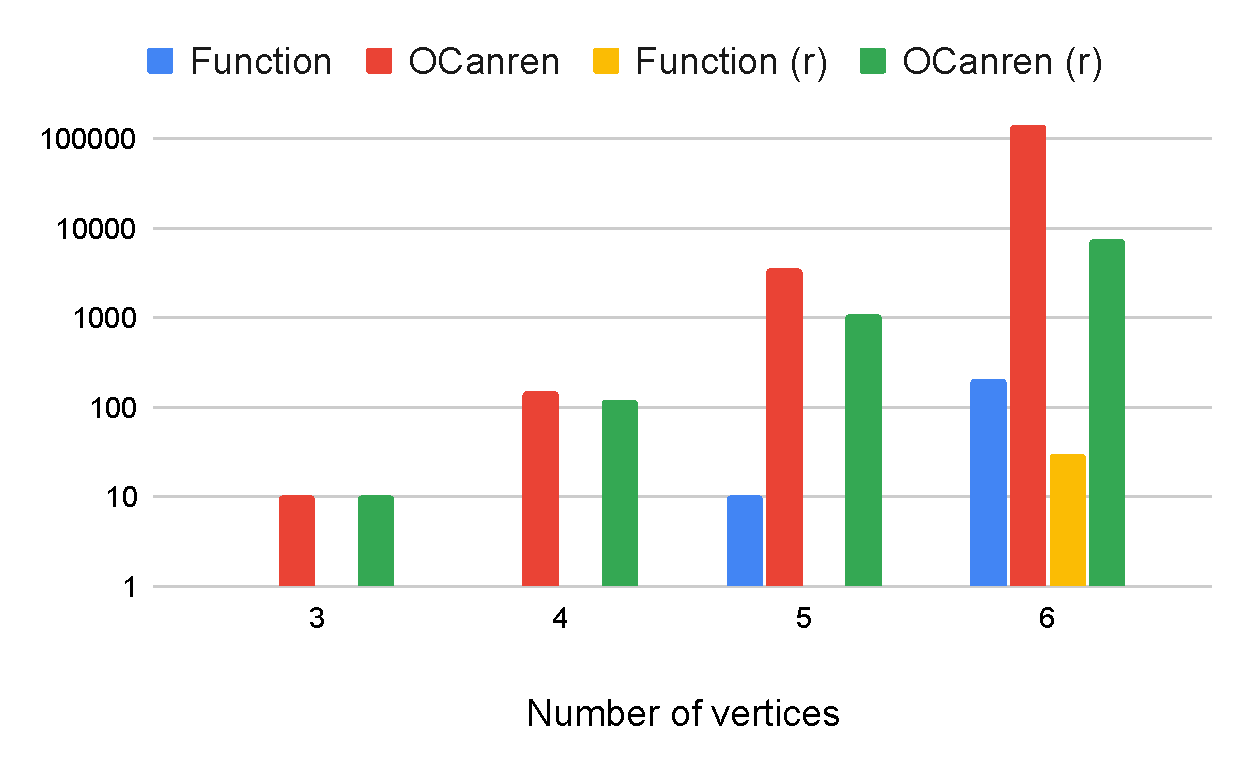
\includegraphics[width=\columnwidth]{fig/eval/topsort.pdf}
  \vspace{-0.7cm}
  \caption{Comparison of exection time of topologic sort (logarithmic scale, time measured in microseconds)}
  \label{graph:topsort}
\end{figure}


\begin{figure}[!h]
  \vspace{-0.5cm}
  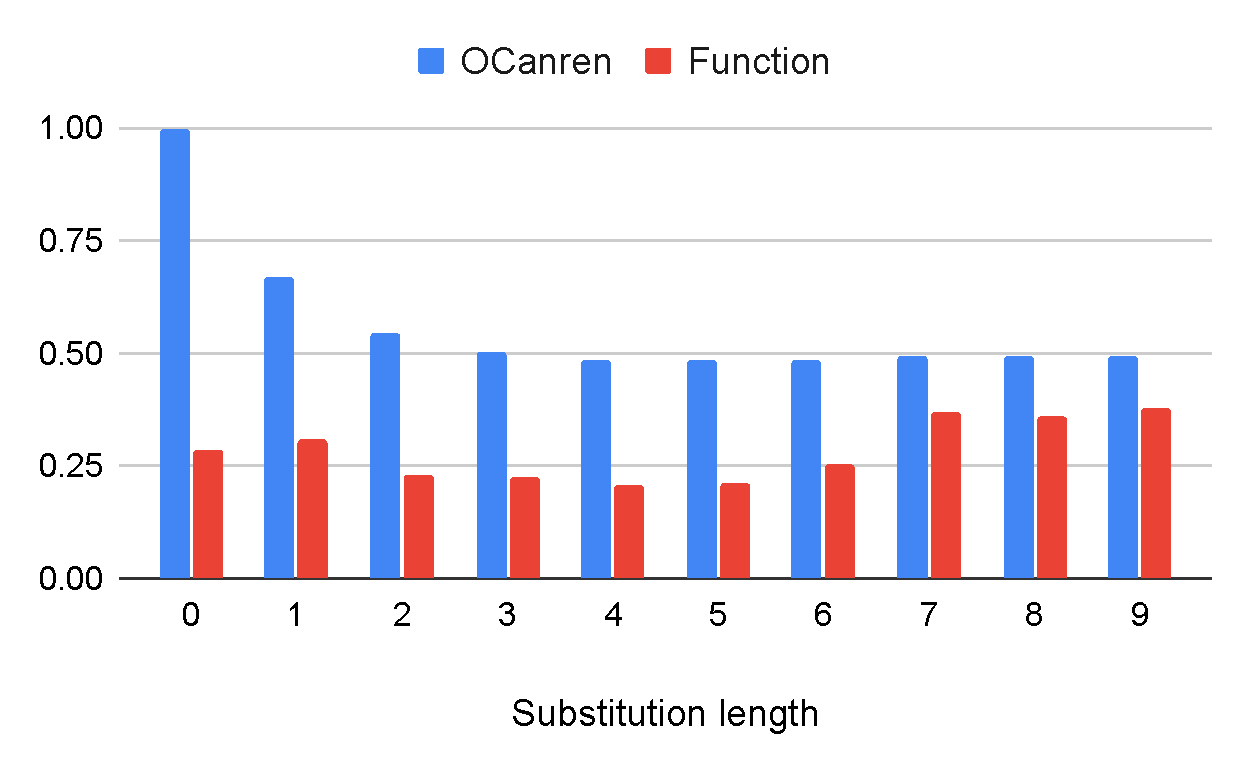
\includegraphics[width=\columnwidth]{fig/eval/prop.pdf}
  \vspace{-0.7cm}
  \caption{Comparison of exection time of formulas generator (time measured in seconds)}
  \label{graph:prop}
\end{figure}




We run \lstinline{topsort$^o$} on directed graphs with exactly one edge between each pair of edges.
For example, graph with 4 vertices has the following edges: \lstinline[breaklines=true]{[(0, 1), (0, 2), (0, 3), (1, 2), (1, 3), (2, 3)]}, which we sort lexicographically.
We generated graphs for a given number of vertices and then executed both relational and functional implementations of \lstinline{topsort$^o$}.
The correct numbering in this condition should map each vertex into itself.
We also run the same functions on the same graph, but with its list of edges reversed, i.e. \lstinline[breaklines=true]{[(2, 3), (1, 3), (1, 2), (0, 3), (0, 2), (0, 1)]}.
In this case, the correct numbering maps a vertex \lstinline{i} into \lstinline{n - i}, where \lstinline{n} is the number of vertices in the graph.

Execution times averaged over 10 runs are presented in table~\ref{tbl:sort} and figure~\ref{graph:topsort}.
Columns ``Functional'' and ``Functional (r)'' contain execution times of functional implementations when run on a graph and reversed graph correspondingly.
Columns ``OCanren'' and ``OCanren (r)'' contain execution times of functional implementations when run on a graph and reversed graph correspondingly.
Relational implementation took more than 300 seconds for a sorted graph with 7 vertices, thus we only consider graphs with up to 6 vertices.
On all graphs, functional implementation is faster than the \mk program.
Topologically sorting a reversed graph takes significantly less time.
This is caused by earlier rejection of candidate solutions, since vertex numbers are higher in the beginning of the list.

As a result of our evaluation, we can conclude that the conversion of \mk program with a given direction into a function speeds up execution a lot and thus it is reasonable to continue working in this direction.


